
\newcommand{\printfigGraphTypes}{
    \begin{figure}
        \begin{subfigure}{.5\textwidth}
            \centering
            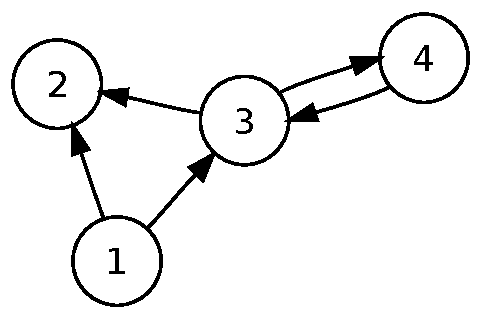
\includegraphics[width=.8\linewidth]{assets/images/Directed_graph_no_background.svg.pdf}
            \caption{Directed graph with cycle between nodes three and four.}
            \label{fig:directedgraph}
        \end{subfigure}
        \begin{subfigure}{.5\textwidth}
            \centering
            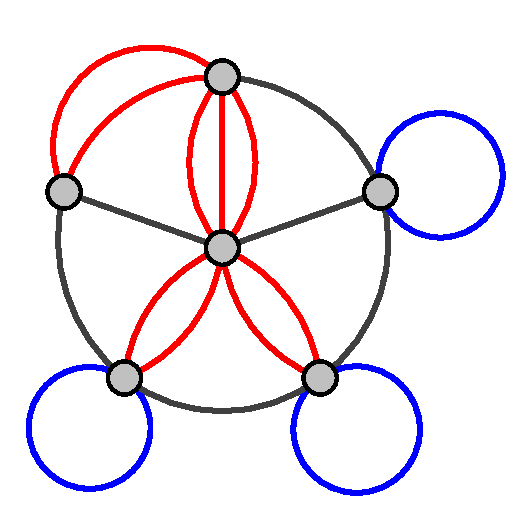
\includegraphics[width=.8\linewidth]{assets/images/Multi-pseudograph.svg.pdf}
            \caption{Multigraph with parallel edges and self-loops}
            \label{fig:multigraph}
        \end{subfigure}%
        \caption[]{Examples of first order graph symantics supported by Jaseci.\footnotemark}
        \label{fig:graph_examples}
    \end{figure}
    \footnotetext{Images credits to wiki contributers~\cite{wiki:Directed_graph_no_background.svg,wiki:Multi-pseudograph.svg}}
}


\newcommand{\printfigHelloWorldBaby}{
    \begin{figure}%{r}{0.5\textwidth}
        \centering
        
\includegraphics[width=.3\linewidth]{assets/images/hello_world_baby.jpg}
        \caption[]{World's youngest coder with valid HTML on shirt.\footnotemark}
        \label{fig:hello_baby}
    \end{figure}
    \footnotetext{Image credit to wiki contributer~\cite{wiki:hello_world_baby.jpg}}
}

\newcommand{\printtabPrecedence}{
    \begin{table}[t]
        \footnotesize
        \centering
        \begin{tabular}{l l l}
            \toprule
            \textbf{Rank} & \textbf{Symbol}                            & \textbf{Description}                           \\
            \midrule
            1             & \texttt{( ), [ ], ., ::, spawn}            & Parenthetical/grouping, node/edge manipulation \\
            2             & \texttt{\textasciicircum, []}              & Exponent,  Index                               \\
            3             & \texttt{*, /, \%  }                        & Multiplication, division, modulo               \\
            4             & \texttt{+, -}                              & Addition, subtraction                          \\
            5             & \texttt{==, !=, >=, <=, >, <, in, not in } & Comparison                                     \\
            6             & \texttt{\&\&, ||, and, or  }               & Logical                                        \\
            7             & \texttt{-->, <--, -[]->, <-[]-}            & Connect                                        \\
            8             & \texttt{=, +=, -=, *=, /=, := }            & Assignment                                     \\
            \bottomrule
        \end{tabular}
        \caption{Precedence of operations in Jac}
        \label{tab:jacprecedence} % Unique label used for referencing the table in-text
        %\addcontentsline{toc}{table}{Table \ref{tab:jacprecedence}} % Uncomment to add the table to the table of contents
    \end{table}
}

\newcommand{\printtabJSAPI}{
    \begin{table}[h]
        \footnotesize

        \begin{tabular}{l p{10cm}}
            \toprule
            \textbf{Interface}  & \textbf{Parameters}                                                                                                   \\
            \midrule
            check loggers       & ()                                                                                                                    \\
            config delete       & (name: str)                                                                                                           \\
            config exists       & (name: str)                                                                                                           \\
            config get          & (name: str)                                                                                                           \\
            config list         & ()                                                                                                                    \\
            config set          & (name: str, value: str, do\_check: bool = True)                                                                       \\
            alias clear         & ()                                                                                                                    \\
            alias delete        & (name: str)                                                                                                           \\
            alias list          & ()                                                                                                                    \\
            alias register      & (name: str, value: str)                                                                                               \\
            architype delete    & (arch: architype, snt: sentinel = None)                                                                               \\
            architype get       & (arch: architype, format: str = 'default', detailed: bool = False)                                                    \\
            architype list      & (snt: sentinel = None, detailed: bool = False)                                                                        \\
            architype register  & (snt: sentinel = None, code: str = `', encoded: bool = False)                                                         \\
            graph active get    & (detailed: bool = False)                                                                                              \\
            graph active set    & (gph: graph)                                                                                                          \\
            graph create        & (set\_active: bool = True)                                                                                            \\
            graph delete        & (gph: graph)                                                                                                          \\
            graph get           & (gph: graph = None, format: str = 'default', detailed: bool = False)                                                  \\
            graph list          & (detailed: bool = False)                                                                                              \\
            graph node get      & (nd: node, ctx: list = None)                                                                                          \\
            graph node set      & (nd: node, ctx: dict, snt: sentinel = None)                                                                           \\
            object get          & (obj: jaseci.element.element, detailed: bool = False)                                                                 \\
            sentinel active get & (detailed: bool = False)                                                                                              \\
            sentinel active set & (snt: sentinel)                                                                                                       \\
            sentinel delete     & (snt: sentinel)                                                                                                       \\
            sentinel get        & (snt: sentinel = None, format: str = 'default', detailed: bool = False)                                               \\
            sentinel list       & (detailed: bool = False)                                                                                              \\
            sentinel register   & (name: str, code: str = '', encoded: bool = False, auto\_run: str = 'init', ctx: dict = {}, set\_active: bool = True) \\
            walker delete       & (wlk: walker.walker, snt: sentinel = None)                                                                            \\
            walker execute      & (wlk: walker.walker)                                                                                                  \\
            walker get          & (wlk: walker.walker, format: str = 'default', detailed: bool = False)                                                 \\
            walker list         & (snt: sentinel = None, detailed: bool = False)                                                                        \\
            walker prime        & (wlk: walker.walker, nd: node = None, ctx: dict = {})                                                                 \\
            walker register     & (snt: sentinel = None, code: str = '', encoded: bool = False)                                                         \\
            walker run          & (name: str, nd: node = None, ctx: dict = {}, snt: sentinel = None)                                                    \\
            walker spawn        & (name: str, snt: sentinel = None)                                                                                     \\
            walker unspawn      & (wlk: walker.walker)                                                                                                  \\

            \bottomrule
        \end{tabular}
        \caption{Precedence of operations in Jac}
        \label{tab:jsAPI}
        %\addcontentsline{toc}{table}{Table \ref{tab:jacprecedence}} % Uncomment to add the table to the table of contents
    \end{table}
}